\documentclass{beamer}
\usepackage[utf8]{inputenc}

\usetheme{Madrid}
\usecolortheme{default}
\usepackage{amsmath,amssymb,amsfonts,amsthm}
\usepackage{mathtools}
\usepackage{txfonts}
\usepackage{tkz-euclide}
\usepackage{listings}
\usepackage{adjustbox}
\usepackage{array}
\usepackage{gensymb}
\usepackage{tabularx}
\usepackage{gvv}
\usepackage{lmodern}
\usepackage{circuitikz}
\usepackage{tikz}
\lstset{literate={·}{{$\cdot$}}1 {λ}{{$\lambda$}}1 {→}{{$\to$}}1}
\usepackage{graphicx}

\setbeamertemplate{page number in head/foot}[totalframenumber]

\usepackage{tcolorbox}
\tcbuselibrary{minted,breakable,xparse,skins}



\definecolor{bg}{gray}{0.95}
\DeclareTCBListing{mintedbox}{O{}m!O{}}{%
  breakable=true,
  listing engine=minted,
  listing only,
  minted language=#2,
  minted style=default,
  minted options={%
    linenos,
    gobble=0,
    breaklines=true,
    breakafter=,,
    fontsize=\small,
    numbersep=8pt,
    #1},
  boxsep=0pt,
  left skip=0pt,
  right skip=0pt,
  left=25pt,
  right=0pt,
  top=3pt,
  bottom=3pt,
  arc=5pt,
  leftrule=0pt,
  rightrule=0pt,
  bottomrule=2pt,
  toprule=2pt,
  colback=bg,
  colframe=orange!70,
  enhanced,
  overlay={%
    \begin{tcbclipinterior}
    \fill[orange!20!white] (frame.south west) rectangle ([xshift=20pt]frame.north west);
    \end{tcbclipinterior}},
  #3,
}
\lstset{
    language=C,
    basicstyle=\ttfamily\small,
    keywordstyle=\color{blue},
    stringstyle=\color{orange},
    commentstyle=\color{green!60!black},
    numbers=left,
    numberstyle=\tiny\color{gray},
    breaklines=true,
    showstringspaces=false,
}

\numberwithin{equation}{section}
\lstset{
  language=Python,
  basicstyle=\ttfamily\small,
  keywordstyle=\color{blue},
  stringstyle=\color{orange},
  numbers=left,
  numberstyle=\tiny\color{gray},
  breaklines=true,
  showstringspaces=false
}


\title{Problem 4.12.44}
\author{Sarvesh Tamgade}

\date{\today} 
\begin{document}

\begin{frame}
\titlepage
\end{frame}

\section{Question}
\begin{frame}{Question}
\textbf{Question}:
Find the equation of the set of points which are equidistant from the points \(\vec{A} = \myvec{1 \\ 2 \\ 3}\) and \(\vec{B} = \myvec{3 \\ 2 \\ -1}\).

\end{frame}

\section{Solution}
\begin{frame}[fragile]
    \frametitle{Solution}
\textbf{Solution:} \
Let \(\vec{X}\) be the position vector of any point equidistant from \(\vec{A}\) and \(\vec{B}\).
The equidistance condition is
\begin{align}
\|\vec{X} - \vec{A}\| = \|\vec{X} - \vec{B}\|.
\end{align}
Squaring both sides, we have
\begin{align}
(\vec{X} - \vec{A})^\top (\vec{X} - \vec{A}) = (\vec{X} - \vec{B})^\top (\vec{X} - \vec{B}).
\end{align}
Expanding and simplifying,
\begin{align}
\vec{X}^\top \vec{X} - 2 \vec{A}^\top \vec{X} + \vec{A}^\top \vec{A} = \vec{X}^\top \vec{X} - 2 \vec{B}^\top \vec{X} + \vec{B}^\top \vec{B},
\end{align}
which reduces to
\begin{align}
-2 \vec{A}^\top \vec{X} + \vec{A}^\top \vec{A} = -2 \vec{B}^\top \vec{X} + \vec{B}^\top \vec{B}.
\end{align}
Rearranging,
\begin{align}
2 (\vec{B} - \vec{A})^\top \vec{X} = \vec{B}^\top \vec{B} - \vec{A}^\top \vec{A}.
\end{align}
Calculate the vector difference:

\end{frame}



\begin{frame}[fragile]
    \frametitle{Solution}
\begin{align}
\vec{B} - \vec{A} = \myvec{3 - 1 \\ 2 - 2 \\ -1 - 3} = \myvec{2 \\ 0 \\ -4} = 2 \myvec{1 \\ 0 \\ -2}.
\end{align}
Calculate the scalar values:
\begin{align}
\vec{B}^\top \vec{B} = 3^2 + 2^2 + (-1)^2 = 14, \quad \vec{A}^\top \vec{A} = 1^2 + 2^2 + 3^2 = 14,
\end{align}
so the right side is zero:
\begin{align}
\vec{B}^\top \vec{B} - \vec{A}^\top \vec{A} = 0.
\end{align}
Thus, substituting the simplified difference vector, the plane equation becomes:
\begin{align}
4\myvec{1 & 0 & -2}\vec{X} = 0,
\end{align}
or equivalently,
\begin{align}
\myvec{1 & 0 & -2}\vec{X} = 0.
\end{align}
\end{frame}
\begin{frame}[fragile]
    \frametitle{Solution}

\textbf{Final Answer:} The set of points equidistant from \(\vec{A}\) and \(\vec{B}\) lies on the plane defined by
\[
\boxed{
\myvec{1 & 0 & -2} \vec{x} = 0
}
\]


\end{frame}
\section{Graph}
\begin{frame}
    \frametitle{Graph}
    \begin{figure}[htbp]
    \centering
    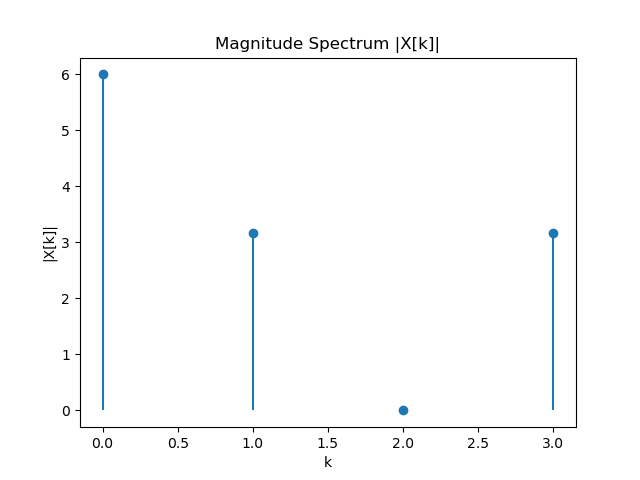
\includegraphics[width=0.65\linewidth]{FIG/fig1.png}
    \caption{Vector Representation}
    \label{fig:FIG/fig1.png}
\end{figure}
\end{frame}
\section{ C Code}
\begin{frame}[fragile]
\frametitle{C Code }
\begin{lstlisting}[language=C]
#include <stdio.h>
#include "matfun.h"

int main() {
    double A[3] = {1, 2, 3};
    double B[3] = {3, 2, -1};
    double BA[3];
    double rhs;

    // Compute B - A
    vector_subtract(B, A, BA, 3);

    // Compute dot products B.B and A.A
    double BTB = dot_product(B, B, 3);
    double ATA = dot_product(A, A, 3);

    rhs = BTB - ATA;


    
\end{lstlisting}
\end{frame}
\begin{frame}[fragile]
\frametitle{C Code }
\begin{lstlisting}[language=C]

    // Multiply BA by 2
    scalar_multiply(BA, BA, 2, 3);

    printf("Vector (2(B - A)) is: [%.2f, %.2f, %.2f]\n", BA[0], BA[1], BA[2]);
    printf("Right-hand side value (B.B - A.A): %.2f\n", rhs);

    printf("Equation of the plane in vector form: [%.2f %.2f %.2f] \\cdot X = %.2f\n", BA[0], BA[1], BA[2], rhs/2);

    return 0;
}


    
\end{lstlisting}
\end{frame}


\begin{frame}[fragile]
\frametitle{Python Code for Plotting}
\begin{lstlisting}[language=Python]
import numpy as np
import matplotlib.pyplot as plt
from mpl_toolkits.mplot3d import Axes3D

# Create grid for y and z
y_vals = np.linspace(-10, 10, 100)
z_vals = np.linspace(-10, 10, 100)
Y, Z = np.meshgrid(y_vals, z_vals)

# Calculate corresponding x using the plane equation: x = 2z
X = 2 * Z

fig = plt.figure()
ax = fig.add_subplot(111, projection='3d')


\end{lstlisting}

\end{frame}
\begin{frame}[fragile]
\frametitle{Python Code for Plotting}
\begin{lstlisting}[language=Python]


# Plot the plane
ax.plot_surface(X, Y, Z, alpha=0.5, color='cyan', edgecolor='k')

# Set axis labels with x, y, z
ax.set_xlabel('x')
ax.set_ylabel('y')
ax.set_zlabel('z')
ax.set_title('3D Plot of plane: x - 2z = 0')
plt.savefig("fig1.png")
plt.show()

\end{lstlisting}

\end{frame}
\begin{frame}[fragile]
\frametitle{Python Code - Using Shared Object}
\begin{lstlisting}[language=Python]
import ctypes
import numpy as np
import matplotlib.pyplot as plt
from mpl_toolkits.mplot3d import Axes3D

# Load the shared library
matfun = ctypes.CDLL('./matfun.so')

# Define argument and return types
matfun.vector_subtract.argtypes = [
    np.ctypeslib.ndpointer(dtype=np.float64),
    np.ctypeslib.ndpointer(dtype=np.float64),
    np.ctypeslib.ndpointer(dtype=np.float64),
    ctypes.c_int
]
matfun.dot_product.argtypes = [
    np.ctypeslib.ndpointer(dtype=np.float64),
    np.ctypeslib.ndpointer(dtype=np.float64),
    
\end{lstlisting}

\end{frame}
\begin{frame}[fragile]
    \frametitle{Python Code - Using Shared Object}
    \begin{lstlisting}
    ctypes.c_int
]
matfun.dot_product.restype = ctypes.c_double
matfun.scalar_multiply.argtypes = [
    np.ctypeslib.ndpointer(dtype=np.float64),
    np.ctypeslib.ndpointer(dtype=np.float64),
    ctypes.c_double,
    ctypes.c_int
]

# Define points A and B
A = np.array([1.0, 2.0, 3.0])
B = np.array([3.0, 2.0, -1.0])

BA = np.zeros(3)
rhs = 0.0
\end{lstlisting}
\end{frame}

\begin{frame}[fragile]
    \frametitle{Python Code - Using Shared Object}
    \begin{lstlisting}
# Compute B - A using shared lib
matfun.vector_subtract(B, A, BA, 3)

# Compute dot products B.B and A.A using shared lib
rhs = matfun.dot_product(B, B, 3) - matfun.dot_product(A, A, 3)

# Calculate 2*(B - A)
BA2 = np.zeros(3)
matfun.scalar_multiply(BA, BA2, 2, 3)

print(f"Vector 2(B - A): {BA2}")
print(f"RHS (B.B - A.A): {rhs}")

# Create grid for y and z
y_vals = np.linspace(-10, 10, 100)
z_vals = np.linspace(-10, 10, 100)
Y, Z = np.meshgrid(y_vals, z_vals)
\end{lstlisting}
\end{frame}
\begin{frame}[fragile]
    \frametitle{Python Code - Using Shared Object}
    \begin{lstlisting}
# From plane equation 2(B - A)^T X = rhs
# Which is BA2^T * X = rhs
# BA2 = [4, 0, -8], so the equation is 4x - 8z = 0
# => x = 2z

# Calculate corresponding x using x = 2z
X = 2 * Z

fig = plt.figure()
ax = fig.add_subplot(111, projection='3d')

# Plot the plane surface
ax.plot_surface(X, Y, Z, alpha=0.5, color='cyan', edgecolor='k')

\end{lstlisting}
\end{frame}
\begin{frame}[fragile]
    \frametitle{Python Code - Using Shared Object}
    \begin{lstlisting}

ax.set_xlabel('x')
ax.set_ylabel('y')
ax.set_zlabel('z')
ax.set_title('3D Plot of plane: x - 2z = 0 (from shared library)')
plt.savefig("fig2.png")
plt.show()

\end{lstlisting}
\end{frame}

\begin{frame}{Plot-Using Both C and Python}
    \centering
    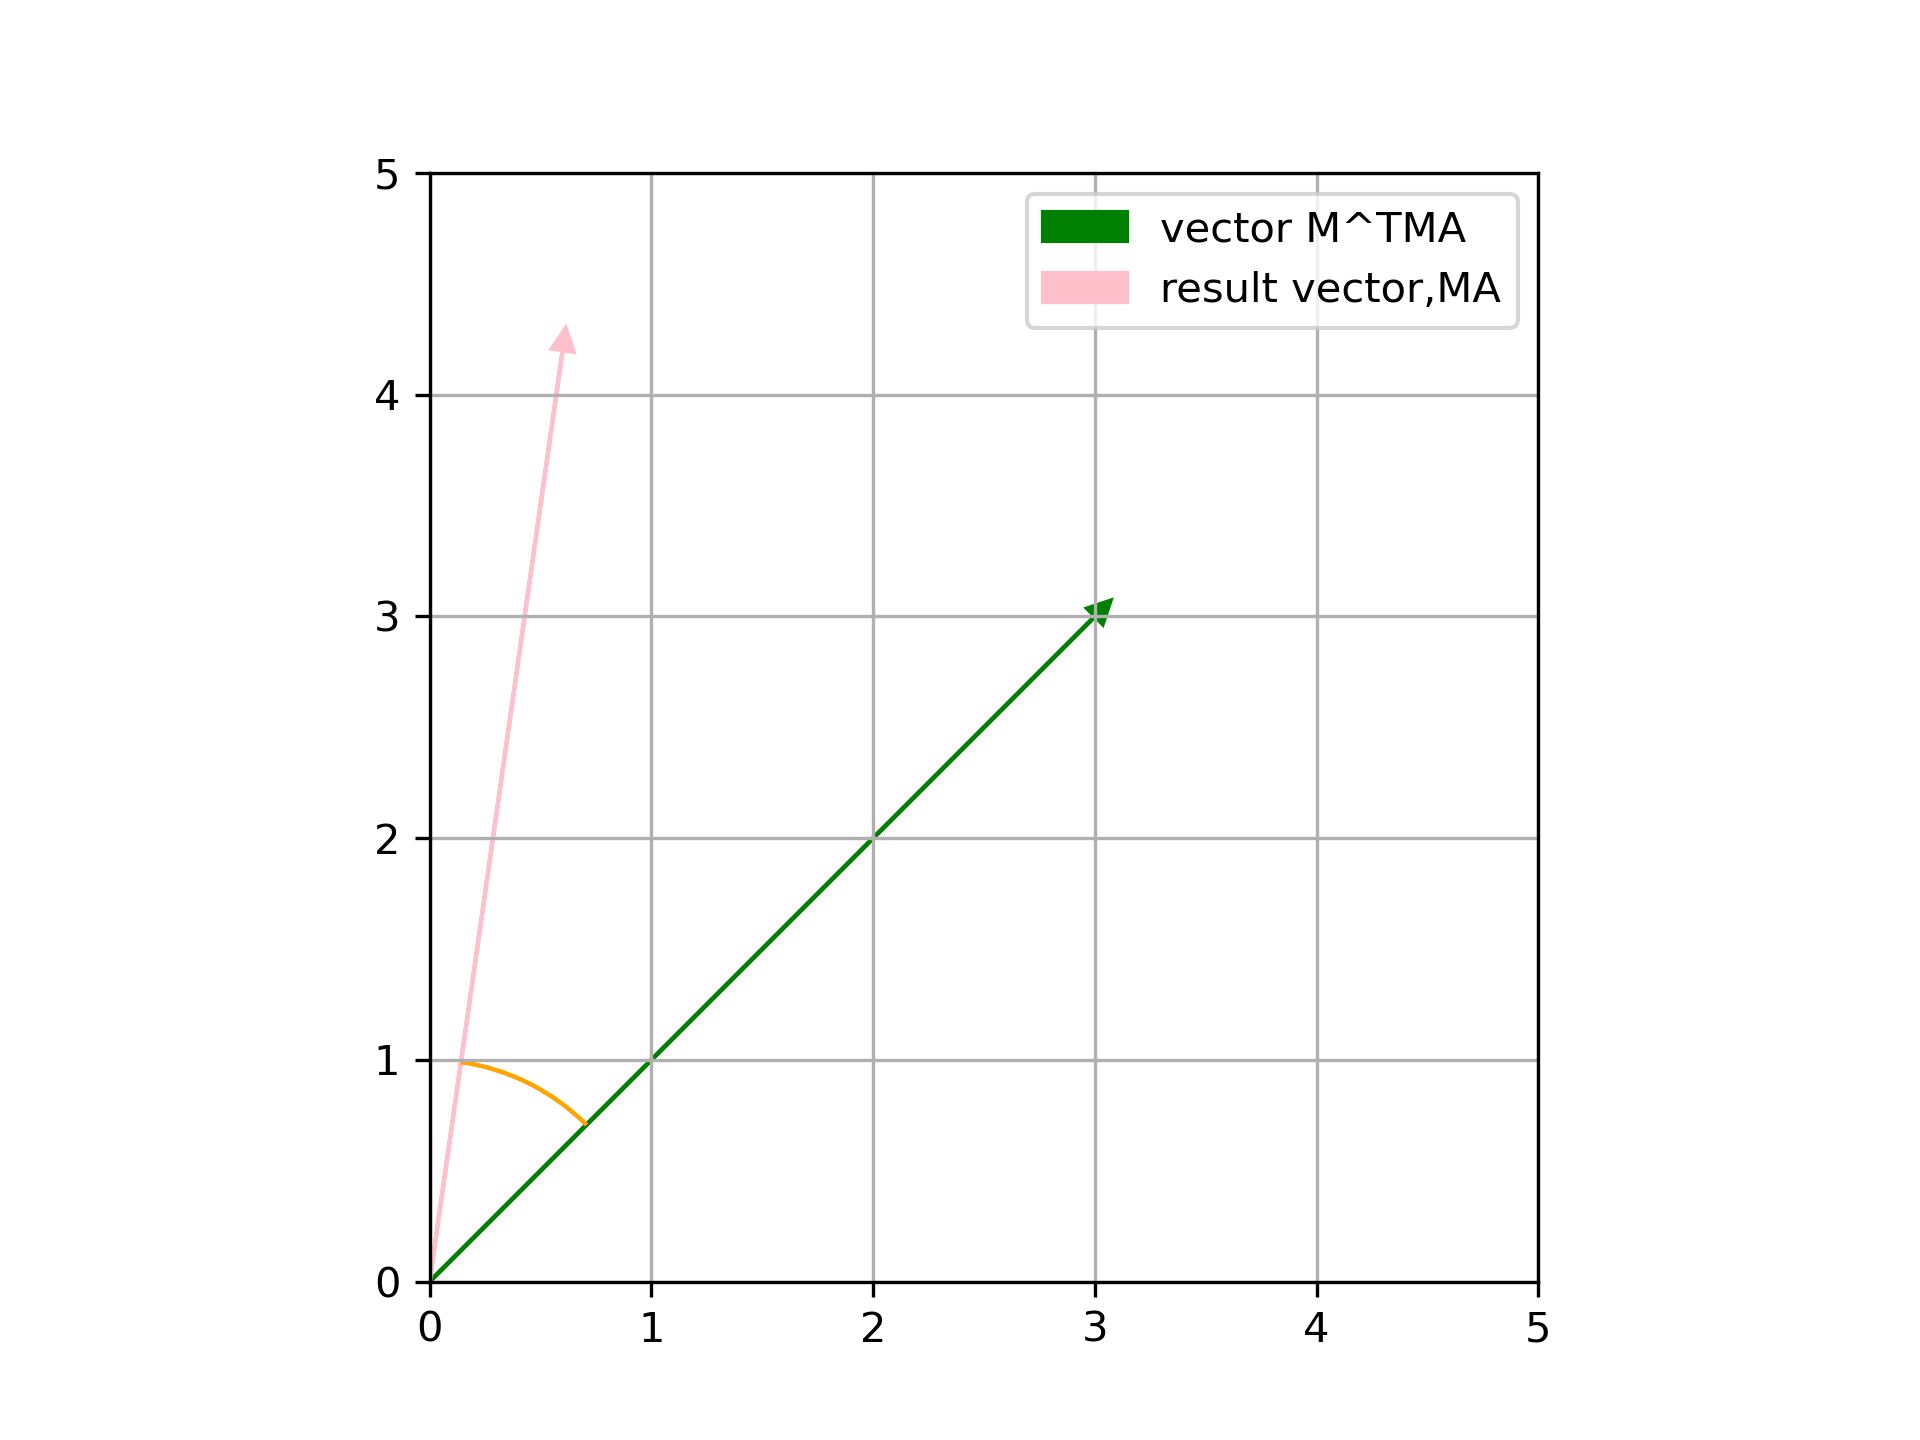
\includegraphics[width=\columnwidth, height=0.8\textheight, keepaspectratio]{FIG/fig2.png}     
\end{frame}


\end{document}
